\section{Glossary}

In this chapter, basic terms will defined and explained.

\subsection{TCP/IP Conceptional Layers}

\begin{enumerate}
      \item \textit{Application:} Standardizes communication interfaces built on Transport Layer protocols for specific classes of applications.\\
            \textbf{Protocols:} \ac{HTTP}, \ac{SSH}, \ac{DNS}, \ac{DHCP}, \ac{NTP}, \ac{POP3}, \ac{IMAP}, \ac{SMTP}, \ac{SSL}/\ac{TLS} (...)
      \item \textit{Transport:} Provide process-to-process communication for application using ports. Features which might be given depending on the protocol are connection-oriented communication, reliability, error correction, flow-control and multiplexing (e.g. multicast / broadcast).\\
            \textbf{Protocols:} \ac{TCP}, \ac{UDP} (...)
      \item \textit{Internet:} Routing and transmission from source to destination.\\
            \textbf{Protocols:} \ac{IP} (v4, v6) (...)
      \item \textit{Network Interface:} Transmission of data between two computers in the same network via physical connection.\\
            \textbf{Protocols:} \ac{MAC}, Tunnels, \ac{PPP} (...)
\end{enumerate}

\subsection{Datagram}

A datagram is a basic transfer unit in a packet-switched network. Datagrams consist of a header and payload. They contain address information and can be send in connectionsless communication.

\subsection{UDP}

The \ac{UDP} provides a simple connectionless communication model. It provides checksums for verification of data integrity and port numbers for addressing specific services on the target machine. It does not have handshaking dialogues and requires no previous packets to be send prior to communication. Messages are mapped directly to packets and are not split up into peaces. \ac{UDP} does not provide a guarantee of delivery, order of packets, or duplicate protection. It therefore exposes the application layer to any unreliability of the network for the sake of less communication overhead. It is suitable for applications which do not require reliability but do require speed e.g. in video streaming or for applications which handle resubmission, ordering and duplicate checking themselves.

\subsection{TCP}

The \ac{TCP} follows a connection-oriented communication model providing reliability, ordering and error checking and flow-control (not allowing one side to send too fast). Messages are handled as a stream of bytes which is split into packets of undefined size for transmission.

\begin{enumerate}
      \item \textit{Connection establishment and termination:} The connection is established using a three-way handshake consisting of the packets SYN $\rightarrow$, SYN-ACK $\leftarrow$ and ACK $\rightarrow$. The connection termination is done with a four-way handshake consisting of the packets FIN $\rightarrow$, ACK $\leftarrow$, FIN $\leftarrow$ and ACK $\rightarrow$. It is possible to shorten this by sending a FIN-ACK as a reply to the FIN
      \item \textit{Reliability:} \ac{TCP} uses sequence numbers to identify each byte of data, as shown in figure \ref{fig:tcp_data_transmission}. The sequence number of the first byte is randomly chosen by the sender of the first packet in order to defend against TCP sequence prediction attacks. Each \ac{TCP}-packet contains a sequence number and \textendash{} if it is an ACK packet \textendash{} an acknowledgement number. The sequence number of the packet is the sequence number of the first byte send in this message or the sequence number of the last byte send in previous messages in case the payload (data) of the packet has size zero (as for ACK packets). The acknowledgement number is the incremented sequence number of the last byte received. TCP uses cumulative ACKs, which means that an acknowledgement number of $n$ acknowledges all bytes with sequence number $< n$.
      \item \textit{Resubmission:} If a single segment in a stream is lost, then the receiver cannot acknowledge subsequent packets, because of the cumulative acknowledgement semantics. TCP uses two mechanisms to trigger the resubmission of lost packets. The first one is \textit{resubmission on duplicate ACKs}, which means the receiver will send ACKs for every subsequently received packet containing the last sequence number before missing packet. If the sender receives three ACKs for the same packet, it will trigger the resubmission of the missing packet. The other mechanism for resubmission is \textit{timeout-based resubmission}, which means that packets will be resubmitted if they are not acknowledged within a given time frame. After a timeout has been triggered, the timeout for the resubmitted packet will be doubled.
      \item \textit{Flow Control:} \ac{TCP} uses a sliding window flow control protocol. The receiver specifies in the \textit{receive window} field of the packet how many bytes it is able to (or willing to) buffer for this connection. The sender can only send that amount of bytes without receiving an ACK, because the ACK signalizes that bytes up to the given acknowledgement number are out of the buffer. This prevents slower machines being overwhelmed with packets, which is important in the internet, because end devices can be very different.
      \item \textit{Error Detection:} In order to detect submission errors, a checksum field ist concluded. However, most errors are also corrected by protocols of underlying layers such as in the Ethernet frame.
\end{enumerate}

\begin{figure}[h]
      \centering
      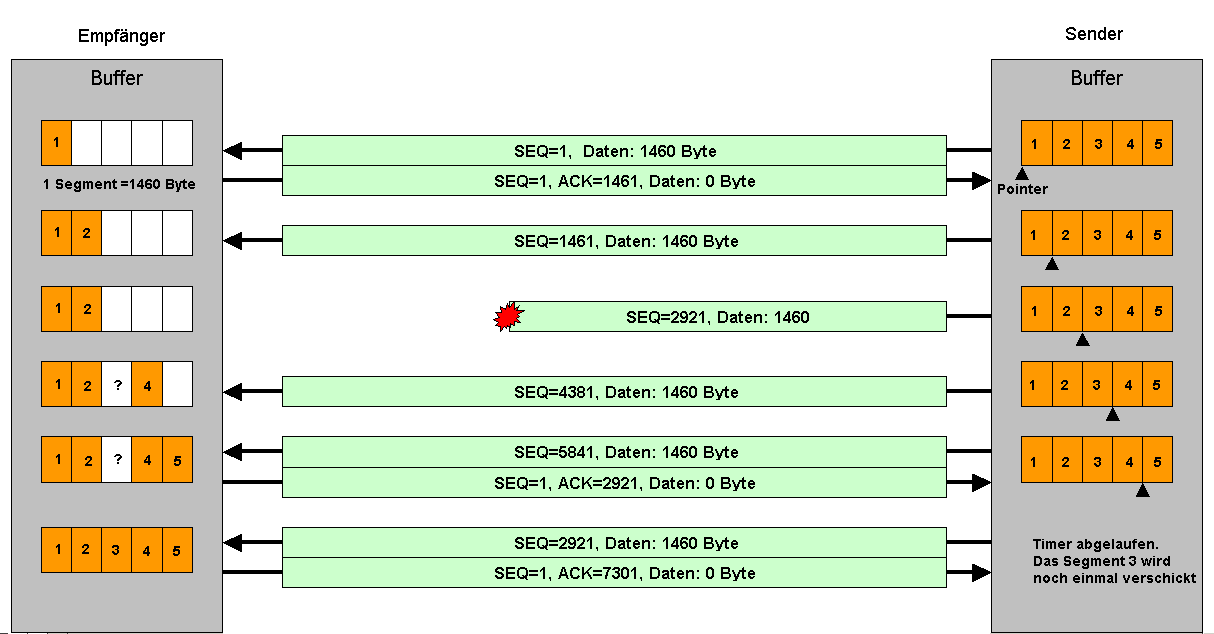
\includegraphics[width=\textwidth]{gfx/Tcp_transfer.png}
      \caption{TCP data transmission with sequence numbers}
      \label{fig:tcp_data_transmission}
\end{figure}

\subsection{Autonomous System}

The internet is a network of computer networks instead of just a huge network of computers. The big networks, which the internet consists of and which are handled independently of their internal structure are called \acp{AS}. This principle allows for scalability, because responsibilities are distributed. In todays world, \acp{AS} are administrative domains hosted by big companies, which commercially offer access to all computers that can be accessed inside or through this system to other \acp{AS}. The routing between \acp{AS} is organized using a so called \ac{EGP}, while routing inside of \acp{AS} is managed using so called \ac{EGP}s. The \ac{EGP} used in todays internet is the \ac{BGP}. For \ac{EGP} the host of the \ac{AS} can choose from multiple protocols such as e.g. \ac{OSPF} or \ac{EIGRP} depending on the internal network topology. Only the edge gateways of an \ac{AS} are responsible for the routing between \acp{AS}, such that internal routers only need to handle internal routing information.

\subsection{Border Gateway Protocol}

The \ac{BGP} is todays \acs{EGP} connecting \acp{AS}. If a new IP address is registered inside of an \ac{AS}, this will be reported to the edge router of the \ac{AS} via an \ac{IGP}. This edge router then transmits the information about the accessibility of this IP address via this \ac{AS} to the edge routers of all other \acp{AS} it is connected to. These edge routers then share this information to all other edge routers of their \ac{AS}, which further share it to other routers of other connected \acp{AS}. As a result, each edge router of an \ac{AS} will know what IP addresses are available inside or behind its own network. They however will no know the exact path, unless the target IP address is located inside of the own \ac{AS}. When a computer inside of one \ac{AS} wants to send a packet to a computer in another \ac{AS}, an \ac{IGP} will lead the packet to the edge router of the \ac{AS}, which will then send it to another suitable \ac{AS}. The receiving edge router then internally routes it to the computer, if it is located in that \ac{AS}, or to another edge router which is connected to other \acp{AS}, which are closer to the destination IP address. This way, routers in an \ac{AS} do not need to know the internal structure of other \acp{AS}, which makes this approach scalable.

\subsection{Round Trip Time}

The \ac{RTT} is the transmission time for a packet from point A to point B plus the transmission time of the ACK-packet from point B back to point A. It can be determined using the ping command.

\subsection{Network Address Translation}

In \ac{IP}v4 there are not enough different IP addresses such that every computer on the world could be assigned a unique address. Therefore the internet is divided into private networks, which form the public network \textendash{} the internet. Inside of private networks, private IP addresses are used, which are unique inside of that private network but not unique for the whole internet. Private IP addresses start with either 10.*, 172.16* or 192.168*. Only the gateway, which connects the private network with the internet, has a public IP address. If a computer inside of a private network wants to connect to a computer outside of that private network, it sends its packet to the default gateway, which is its connection to the public network. The gateway then opens a session for that connection attempt which maps the port of the private host to a given port of the gateway and stores that information in the so called \ac{NAT}-table. It then replaces the private IP address and port with its own public address and the port assigned to that connection and forwards it to its destination (possibly via borders of \acl{AS}s). If the receiver wants to reply to the host in the private network, it sends the reply to the global IP address of the gateway connected to the private network. Then the gateway router looks at the port of the incoming packet and translates the IP address back to the private IP address and port based on the port mapping specified in the \ac{NAT}-table. By the way, this means, that publicly available services must have their own public IP address or receive a dedicated static mapping in order to be available from outside of their private networks. \ac{NAT} is criticized, because it mixes IP addresses with port numbers, which originate from different layers of the \ac{TCP}/\ac{IP} protocol stack \textendash{} the \textit{internet} and the \textit{transport} layer.

\subsection{Subnetting}

Subnetting splits networks into subnets using a so called subnet mask, which divides IP addresses into two parts \textendash{} the network ID and the host ID. Subnetting solves a different issue than \ac{NAT}. While \ac{NAT} increases the address space through mapping multiple private IP addresses to one public IP address, subnetting allows to split networks in order to increase their maintainability and limit the range of broadcast packets. A given private network with private IP addresses can therefore be split up further into multiple subnets, while all host can use the same public IP address. The subnet size, which is defined through the subnet mask, is set by the network administrator. If a host in a subnet wants to send a packet to a specific IP-address it first checks if the host is in the same subnet using the subnet mask and in this case sends it to this host via the best available path possible in the topology of the subnet. Otherwise the packet is sent to the gateway of the subnet, whose network ID is defined through the subnet and host ID is zero. Only in case the IP address is a global IP address, it would be sent all the way up the the upper most gateway, which connects the private network to the internet and translate the private to the public IP address. Therefore \ac{NAT} and subnetting are independent. Subnet masks can be written like an IP address or in the so called CIDR prefix notation, which is the number of 1-bits in subnet mask if written in binary format. I.e. the subnet mask 255.255.255.128 can also be written as /25. A subnet with a given IPv4 CIDR prefix subnet mask has $2^{32 - prefix}$ usable addresses, because this is the amount of numbers the host bits (non-zero bits of the subnet mask) can represent. The address, where all host bits are 1s, is the braodcast address, which will make packets be send to all members of the subnet.
